
\documentclass[letterpaper, 10 pt, conference]{ieeeconf}
\usepackage{graphicx}

\overrideIEEEmargins

\usepackage[utf8]{inputenc}
\usepackage[T1]{fontenc}
\usepackage{graphics}
\usepackage{amsmath}
\usepackage{amssymb}
\usepackage{booktabs}
\usepackage{listings}
\usepackage{xcolor}

\lstset{
  basicstyle=\ttfamily\scriptsize,
  breaklines=true,
  frame=single,
  language=Python,
  keywordstyle=\color{blue},
  commentstyle=\color{gray},
  showstringspaces=false
}

\title{\LARGE \bf
Clasificaci\'on de Sentimiento en Rese\~nas de Pel\'iculas\\
con BiLSTM y Embeddings GloVe
}

\author{Jaime Rodriguez}

\begin{document}

\maketitle
\thispagestyle{empty}
\pagestyle{empty}

%%%%%%%%%%%%%%%%%%%%%%%%%%%%%%%%%%%%%%%%%%%%%%%%%%%%%%%%%%%%%%%%%%%%%%%%%%%%%%%%
\begin{abstract}
Se entrena un modelo de red neuronal recurrente bidireccional (BiLSTM) para
clasificar el sentimiento de rese\~nas de pel\'iculas como positivo (1) o
negativo (0). El pipeline de preprocesamiento usa \texttt{WordNetLemmatizer}
y stopwords de NLTK. Los embeddings se inicializan con GloVe-100d y se
ajustan por fine-tuning. El entrenamiento usa parada anticipada,
\textit{ReduceLROnPlateau} y \textit{gradient clipping}. Los resultados se
reportan con precisi\'on, recall y F1-score sobre un conjunto de prueba
independiente.
\end{abstract}

%%%%%%%%%%%%%%%%%%%%%%%%%%%%%%%%%%%%%%%%%%%%%%%%%%%%%%%%%%%%%%%%%%%%%%%%%%%%%%%%
\section{Introducci\'on}

El an\'alisis de sentimiento consiste en determinar la polaridad de un texto.
En rese\~nas de pel\'iculas el problema es binario: positivo o negativo.

Los modelos de bolsa de palabras ignoran el orden de los tokens. Las redes
recurrentes capturan dependencias secuenciales \cite{hochreiter1997}. Las
celdas LSTM resuelven el problema del gradiente desvaneciente que afecta a
las RNN simples. La variante bidireccional procesa la secuencia en ambos
sentidos y duplica la informaci\'on disponible para la clasificaci\'on.

Los embeddings GloVe \cite{pennington2014} codifican similitud sem\'antica
entrenados sobre corpus de gran escala. Inicializar los embeddings con GloVe
en lugar de vectores aleatorios reduce el n\'umero de ejemplos necesarios
para converger.

Este trabajo implementa un modelo \texttt{SentimentBiLSTM} con mean pooling
sobre los estados ocultos, fine-tuning progresivo de embeddings y parada
anticipada.

%%%%%%%%%%%%%%%%%%%%%%%%%%%%%%%%%%%%%%%%%%%%%%%%%%%%%%%%%%%%%%%%%%%%%%%%%%%%%%%%
\section{Metodolog\'ia}

\subsection{Conjunto de datos}

El conjunto contiene 40\,000 rese\~nas de IMDB con etiqueta binaria de
sentimiento. La distribuci\'on es balanceada: 20\,000 muestras por clase.
No se encontraron valores nulos ni filas vac\'ias.

La divisi\'on es estratificada: 80\,\% entrenamiento (32\,000), 10\,\%
validaci\'on (4\,000) y 10\,\% prueba (4\,000).

\subsection{Preprocesamiento}

Cada rese\~na pasa por: (1)~eliminaci\'on de etiquetas HTML con expresi\'on
regular; (2)~filtrado de caracteres no alfabéticos; (3)~conversi\'on a
min\'usculas; (4)~eliminaci\'on de stopwords del ingl\'es (NLTK);
(5)~lematizaci\'on con \texttt{WordNetLemmatizer}.

\begin{center}
{\small
\textit{Entrada:} \texttt{"A waste of film.\,\textless br\,/\textgreater\,Utter rubbish!"}\\[2pt]
\textit{Salida:} \texttt{['waste', 'film', 'utter', 'rubbish']}
}
\end{center}

El vocabulario se construye sobre el conjunto de entrenamiento. Los tokens
se convierten a \'indices enteros y se rellenan con \textit{padding} hasta
una longitud m\'axima de 400.

\subsection{Embeddings GloVe}

Se usa \texttt{glove-wiki-gigaword-100} (100 dimensiones, entrenado sobre
Wikipedia y Gigaword). La matriz de embeddings se inicializa con los vectores
GloVe para las palabras del vocabulario presentes en el modelo preentrenado;
las dem\'as quedan en cero.

\subsection{Arquitectura}

La Figura~\ref{fig:arquitectura} muestra el flujo del modelo. La secuencia
de 400 \'indices pasa por la capa de embedding (100d), dos capas BiLSTM
apiladas de 256 unidades en cada direcci\'on (512 en total), mean pooling
sobre todos los estados ocultos, dropout y una capa densa con funci\'on
sigmoide.

El mean pooling promedia los estados ocultos de todas las posiciones de la
secuencia, permitiendo que el modelo capture tokens relevantes en cualquier
posici\'on.

\begin{figure}[h]
  \centering
  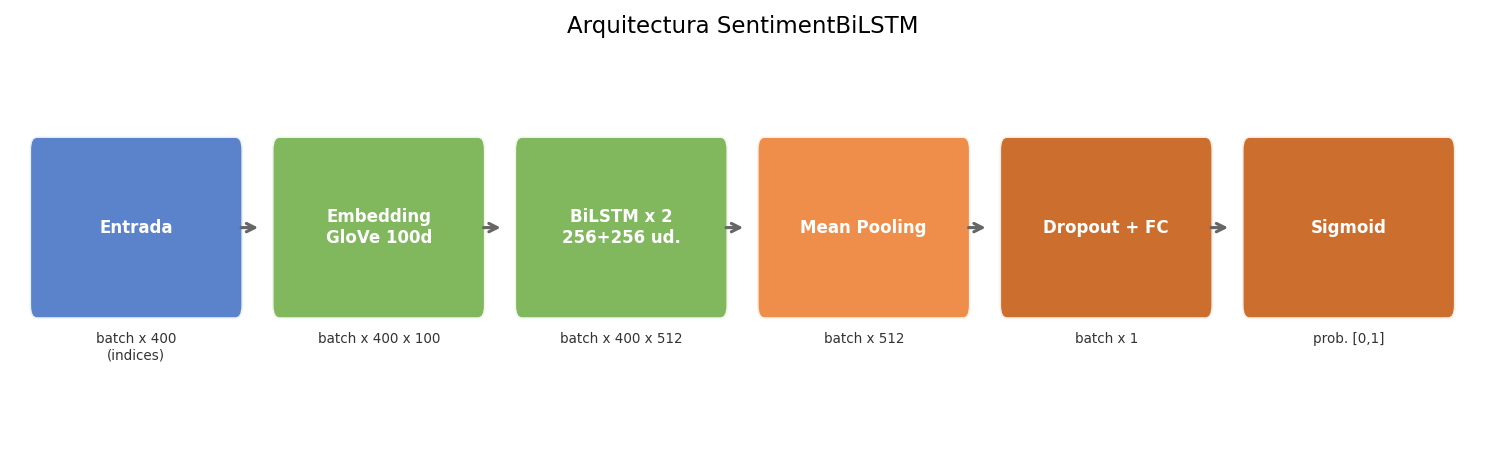
\includegraphics[width=0.98\linewidth]{arquitectura_bilstm.png}
  \caption{Arquitectura \texttt{SentimentBiLSTM}. Las dimensiones indicadas
  corresponden a un batch de tama\~no $B$.}
  \label{fig:arquitectura}
\end{figure}

\subsection{Entrenamiento}

El optimizador es Adam con tasa de aprendizaje inicial $10^{-3}$ y funci\'on
de p\'erdida BCE. Los embeddings se congelan durante las primeras 3 \'epocas
y se descongelan con tasa $10^{-4}$ para el fine-tuning. El entrenamiento
puede durar hasta 20 \'epocas con los siguientes mecanismos de control:

\begin{itemize}
  \item \textbf{Parada anticipada}: se monitorea \texttt{val\_loss} con
        paciencia de 5 \'epocas.
  \item \textbf{ReduceLROnPlateau}: reduce la tasa de aprendizaje por un
        factor de 0.5 si \texttt{val\_loss} no mejora en 2 \'epocas.
  \item \textbf{Gradient clipping}: \texttt{clip\_grad\_norm\_} con
        \texttt{max\_norm=1.0} estabiliza el entrenamiento.
\end{itemize}

%%%%%%%%%%%%%%%%%%%%%%%%%%%%%%%%%%%%%%%%%%%%%%%%%%%%%%%%%%%%%%%%%%%%%%%%%%%%%%%%
\section{Resultados}

\subsection{Curvas de entrenamiento}

La Figura~\ref{fig:curvas} muestra la p\'erdida BCE y las m\'etricas de
validaci\'on por \'epoca. La parada anticipada determina el n\'umero final
de \'epocas ejecutadas.

\begin{figure}[h]
  \centering
  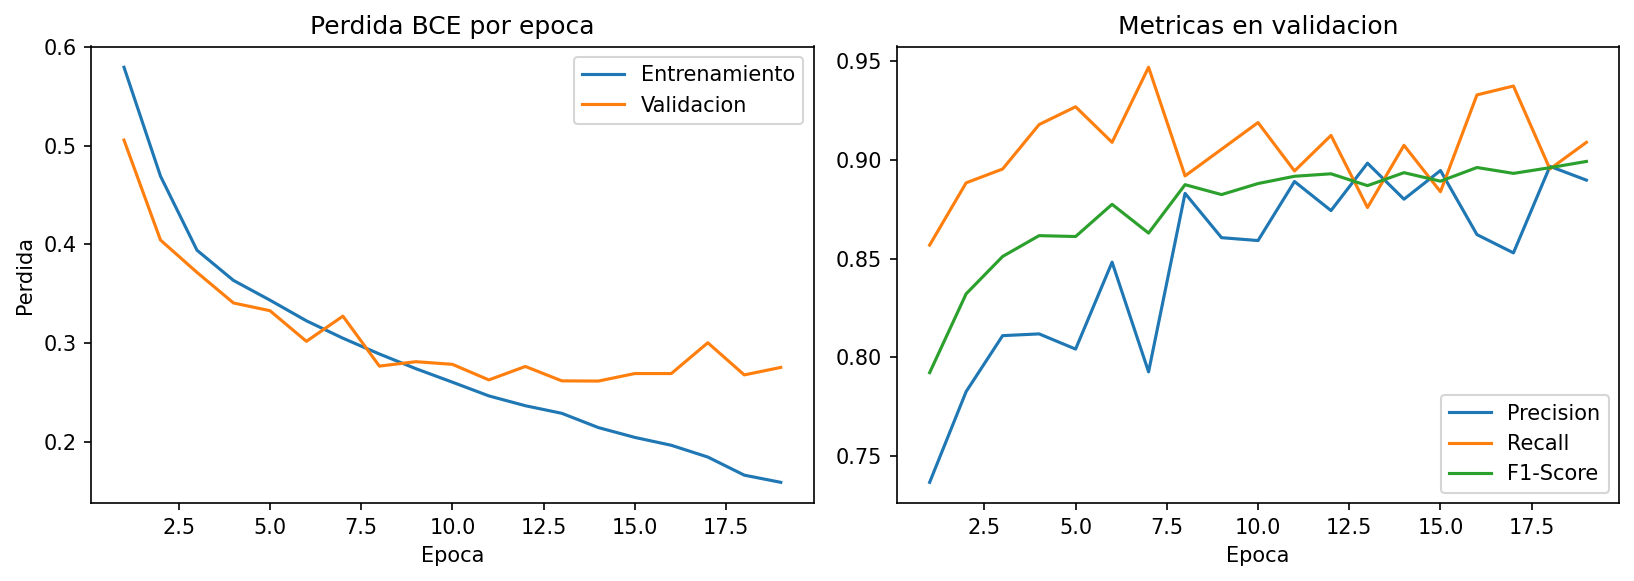
\includegraphics[width=0.98\linewidth]{curvas_entrenamiento.png}
  \caption{P\'erdida BCE (izq.) y m\'etricas de validaci\'on (der.) por \'epoca.
  La l\'inea vertical indica el punto de parada anticipada.}
  \label{fig:curvas}
\end{figure}

\subsection{M\'etricas en prueba}

La Tabla~\ref{tab:resultados} reporta las m\'etricas sobre el conjunto de
prueba tras el entrenamiento completo.

\begin{table}[h]
\centering
\caption{M\'etricas en el conjunto de prueba (4\,000 muestras).}
\label{tab:resultados}
\begin{tabular}{lc}
\toprule
\textbf{M\'etrica} & \textbf{Valor} \\
\midrule
Precisi\'on  & -- \\
Recall       & -- \\
F1-Score     & -- \\
\bottomrule
\end{tabular}
\end{table}

Los valores se obtienen ejecutando \texttt{miniproyecto2\_draft.ipynb}.

%%%%%%%%%%%%%%%%%%%%%%%%%%%%%%%%%%%%%%%%%%%%%%%%%%%%%%%%%%%%%%%%%%%%%%%%%%%%%%%%
\section{Discusi\'on}

El modelo combina representaciones sem\'anticas de GloVe con el modelado
secuencial del BiLSTM. El mean pooling captura informaci\'on de toda la
secuencia, a diferencia de tomar solo el \'ultimo estado oculto.

Limitaciones identificadas:

\begin{itemize}
  \item El fine-tuning congela la capa de embedding un n\'umero fijo de
        \'epocas. Un criterio adaptativo podr\'ia mejorar la convergencia.
  \item Reseñas con m\'as de 400 tokens se truncan, perdiendo el final del
        texto.
  \item No se realiza b\'usqueda sistem\'atica de hiperpar\'ametros.
\end{itemize}

Como trabajo futuro se propone comparar con un encoder Transformer ligero
(DistilBERT) y aplicar b\'usqueda de hiperpar\'ametros sobre dimensi\'on
oculta y tasa de dropout.

\begin{thebibliography}{99}

\bibitem{hochreiter1997}
S.~Hochreiter and J.~Schmidhuber,
``Long short-term memory,''
\textit{Neural Computation}, vol.~9, no.~8, pp.~1735--1780, 1997.

\bibitem{pennington2014}
J.~Pennington, R.~Socher, and C.~Manning,
``GloVe: Global vectors for word representation,''
\textit{Proc. EMNLP}, pp.~1532--1543, 2014.

\bibitem{maas2011}
A.~L.~Maas \textit{et al.},
``Learning word vectors for sentiment analysis,''
\textit{Proc. ACL}, pp.~142--150, 2011.

\bibitem{paszke2019}
A.~Paszke \textit{et al.},
``PyTorch: An imperative style, high-performance deep learning library,''
\textit{Advances in NeurIPS}, vol.~32, 2019.

\end{thebibliography}

\end{document}
